\chapter{Kinematics in Two Dimensions}
	\section{Introduction}
	
	When an object is moving in two (or three) dimensions at once - like when it moves both horizontally and vertically at the same time - the motion of the object in each dimension is completely independent.  This means that each dimension will have its own set of kinematic variables.  The only kinematic variable that can be used in all directions is time, since time is a scalar and does not have a direction.  Thus, instead of only five kinematic variables, problems will have sets of five variables in each direction, with time counting for every dimension.  
	
	
{\renewcommand{\arraystretch}{1.2}
\begin{center}
	
	
	\begin{table}[ht]\caption{\textbf{Kinematic Variables in Multiple Dimensions}}% title of Table 
		\centering % used for centering table	
		\begin{tabular}{|c|c||c|c|}
			\hline \hline
			\textbf{Quantity} & \textbf{Variable} & \textbf{Quantity} & \textbf{Variable}  \\
			\hline
			Horizontal Displacement & $\vec{d_x}$ or $\vec{x}-\vec{x_0}$  & Vertical Displacement & $\vec{d_y}$ or $\vec{y}-\vec{y_0}$ \\
			\hline
		
			Horizontal Initial Velocity & $\vec{v_{ix}}$ or $\vec{v_{0x}}$  & Vertical Initial Velocity & $\vec{v_{iy}}$ or $\vec{v_{0y}}$ \\
\hline

			Horizontal Final Velocity & $\vec{v_{fx}}$ or $\vec{v_x}$  & Vertical Final Velocity & $ \vec{v_{fy}}$ or $\vec{v_y}$ \\ 
	\hline
	Horizontal Acceleration & $\vec{a_x}$  &  Vertical Acceleration & $\vec{a_y} $ \\
	\hline
	\multicolumn{2}{|c|}{Time} & \multicolumn{2}{|c|}{$t$} \\
	\hline
		
		\end{tabular}
		\label{table:kinematic2d}% is used to refer this table in the text
	\end{table}
\end{center}

\section{Projectiles}
\index{Projectiles}

A \textbf{projectile} is any object that meets the following critera:
\begin{itemize}
	\item The object is in \textit{free-fall}.  That is, Gravity is the only force that acts on the object (all other forces are negligable).
	\item The object is moving in two dimensions at the same time.  Most often, describe it as moving both horizontally and vertically at the same time.  
\end{itemize}


\subsection{Horizontally Launched Projectiles}
	\index{Projectiles, Launched Horizontally}
Often, projectiles will be launched horizontally, such as when a ball rolls off a table, or when an archer shoots a perfectly level arrow.  In this case, the math is somewhat easier to deal with.  The initial velocity stated in the problem will be entirely horizontal, and the initial vertical velocity will be zero.


\begin{mdframed}[backgroundcolor=blue!10!white]
	\begin{center}
		
		
		\textbf{Example \thesection.1}	
	\end{center}
	
	\textbf{Problem: } A ball is rolling 2.1 m/s when it rolls off the edge of a 1.3 meter high table.
	\begin{enumerate}
		\item How long is the ball in the air?
		\item How far, horizontally, does the ball land from the edge of the table?
		\item What is the magnitude of the final velocity of the ball?
		\item What is the angle of impact?
	\end{enumerate}
	\vspace{0.1in}
	
	\textbf{Solution:} 
	Begin by drawing a diagram:
	
	\begin{tikzpicture}
		% Draw the table
		%\draw[thick] (0,0) rectangle (1,-1.3);
		%\node at (0.5, -1.4) [below] {Table (1.3 m)};
		
		% Draw the ball's initial position
		\filldraw[black] (0.5,0) circle (0.1);
		%\node at (0.4, 0) [left] {Ball};
		
		% Draw the trajectory of the ball
		\draw[->, thick, dashed] (0.5,0) .. controls (3.5,-1) and (5,-2.5) .. (6,-3.3);
		
		 Draw initial velocity components
		\draw[->, thick, red] (0.5,0) -- (2,0);
		\node at (1.25,0) [above,red] {$v_{0} = 2.1\, \text{m/s}$};
		
		% Draw initial downward velocity
		%\draw[->, thick, blue] (0.5,0) -- (0.5,-0.8);
		%\node at (0.5,-0.4) [left] {$v_y = 0\, \text{m/s}$};
		
		% Draw horizontal and vertical distance markers
		\draw[|-|] (6,0) -- (6,-3.3);
		\node at (6.6,-1.65) [right] {$y-y_0 = \SI{1.3} {m}$};
		
		\draw[|-|] (0.5,-3.3) -- (6,-3.3);
		\node at (3.25,-3.6) [below] {$x-x_0$};
		
		%Draw the coordinate system
			\draw[->,blue] (-1.5,1) -- (-1.5,0.5);
		\node at (-1.5,0.4) [below,blue] {+y};
		
			\draw[->,blue] (-1.5,1) -- (-1,1);
			\node at (-0.9,1) [right,blue] {+x};

		
		% Final velocity and angle markers
		%\draw[->, thick, green] (6,-3.3) -- (6.5,-4);
		%\node at (6.5,-3.6) [right] {$\vec{v}$};
		
		%\draw[->] (6,-3.3) -- (7,-3.3);
		%\node at (7,-3.3) [above] {$v_x$};
		
		%\draw[->] (6,-3.3) -- (6,-4.5);
		%\node at (6,-4.5) [left] {$v_y$};
		
		% Draw angle of impact
		%\draw (6,-3.3) arc[start angle=-90, end angle=-60, radius=1];
		%\node at (6.8,-3.8) {$\theta$};
		
	\end{tikzpicture}
	
	You may notice from the coordinate system that the downward direction has been chosen as +y.  This will help us to avoid needing negatives in the problem.
	
	Next, we create a table with each of the kinematic variables for each dimension:
	
	\begin{longtable}{|c l | c l|}
		\hline
		\multicolumn{2}{|c|}{\textbf{Horizontal}} & \multicolumn{2}{|c|}{\textbf{ Vertical}} \\
		\hline
		$\vec{x}-\vec{x_0}$ =&     & $\vec{y}-\vec{y_0} = $ & $\SI{1.3}{m}$ \\
		\hline
		$\vec{v_{0x}} = $ & $\SI{2.1}{m/s}$ & $\vec{v_{0y}} = $ & $\SI{0}{m/s}$ \\
		\hline
		$v_x = $&  & $v_y = $ &  \\
		\hline
		$a_x = $ & $\SI{0}{m/s^2}$ & $a_y = $ & $\SI{9.81}{m/s^2}$ \\ 
		\hline
		\multicolumn{2}{|r}{$t = $} & \multicolumn{2}{l|}{  }  \\
		\hline
	\end{longtable}
	
	\begin{enumerate}
		\item We see that the vertical direction has three variables, and can be used to calculate the time the ball is in the air, using equation \cref{equation:kinematic3}, applied in the vertical direction: 
		\begin{equation*}
			y - y_0 = \cancelto{0}{v_{0y}t} + \frac{1}{2}a_yt^2
		\end{equation*}

	Solving for t yields:
		\begin{equation*}
		t = \sqrt{\frac{2(y-y_0)}{a_y}} = \sqrt{\frac{2(\SI{1.3}{m})}{\SI{9.81}{m/s^2}}} \approx \SI{0.515}{s}
	\end{equation*}

	\item To find the distance the ball has traveled horizontally, we can use the same kinematic equation as the previous step, only this time, applied in the horizontal direction:
	\begin{equation*}
	x - x_0 = v_{0x}t + \cancelto{0}{\frac{1}{2}a_xt^2}
\end{equation*}

	\begin{equation*}
	x - x_0 = (\SI{2.1}{m/s})(\SI{0.515}{s})  \approx \SI{1.081}{m}
\end{equation*}
\item Finding the final velocity of the ball requires finding both the x- and y- components of the final velocity:
	\begin{equation*}
	v_x = v_{0x} + \cancelto{0}{a_x t} = \SI{2.1}{m/s}
\end{equation*}

	\begin{equation*}
	v_y = \cancelto{0}{v_{0y}} + a_y t = \SI{9.81}{m/s^2} \SI{0.515}{s} \approx \SI{5.050}{m/s}
\end{equation*}
	
	
	We can use these components of the final velocity to determine v according to the following diagram:
	
	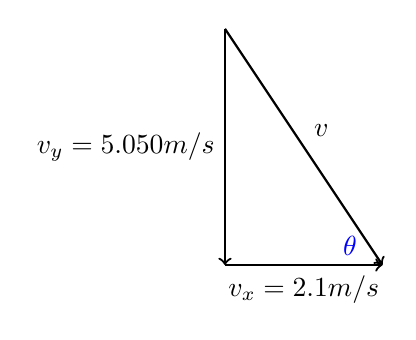
\begin{tikzpicture}
		% Draw the vertical side (v_x)
		\draw[->, thick] (0,0) -- (0,-3) node[midway, left] {$v_y = \SI{5.050}{m/s}$};
		
		% Draw the horizontal side (v_y)
		\draw[->, thick] (0,-3) -- (2,-3) node[midway, below] {$v_x = \SI{2.1}{m/s}$};
		
		% Draw the hypotenuse (v)
		\draw[->, thick] (0,0) -- (2,-3) node[midway, above right] {$v$};
		
		\node at (1.8,-3) [above left,blue] {$\theta$};
		
	\end{tikzpicture}

		Using the pythagorean theorum, we find:
			\begin{equation*}
			v = \sqrt{v_x^2 + v_y^2} = \sqrt{(\SI{2.1}{m/s})^2+(\SI{5.050}{m/s})^2} \approx \SI{5.470}{m/s}
		\end{equation*}
	
	\item The angle of impact is marked as \color{blue} $\theta$ \color{black} in the diagram for part 3.  We can find the angle of impact by using trigonometry.  Using tangent yields:
	
			\begin{equation*}
	\tan {\theta} = \frac{opp}{adj} 
	\end{equation*}

	\begin{equation*}
	\theta = \tan^{-1} (\frac{opp}{adj}) = \tan^{-1} (\frac{v_y}{v_x}) = \tan^{-1} (\frac{\SI{5.050}{m/s}}{\SI{2.1}{m/s}}) \approx 67.420 \degree
	\end{equation*}

		
	\end{enumerate}

	
\end{mdframed}	
	
	
	
	
	
	\subsection{Projectiles Launched at an Arbitrary Angle}
	\index{Projectiles, Launched at an Arbitrary Angle}
	\subsubsection{Projectiles Launched at an Arbitrary Angle on Level Ground}
	\subsubsection{Projectiles Launched at an Arbitrary Angle on Uneven Ground}
	\subsubsection{Projectiles Launched at an Arbitrary Angle Near a Mountain or Hill}
		
		


	


